\documentclass{article}
\usepackage[T1]{fontenc}
\usepackage[utf8]{inputenc}
\usepackage[x11names]{xcolor}
\usepackage{lipsum}

\usepackage{titlesec}
\usepackage[utf8]{inputenc} %page number

\usepackage{graphicx}

\usepackage{fancyhdr}

\usepackage[letterpaper, landscape, margin=1in]{geometry}
\usepackage{xcolor}

\usepackage[colorlinks = true,
            linkcolor = blue,
            urlcolor  = blue,
            citecolor = blue,
            anchorcolor = blue]{hyperref}

\newcommand{\MYhref}[3][blue]{\href{#2}{\color{#1}{#3}}}%

\graphicspath{ {images/}} %picture


\titleformat{\section}
{\normalfont\huge\bfseries}{\thesection}{1em}{}
\titleformat{\subsection}
{\normalfont\large\bfseries}{\thesubsection}{1em}{}
\titleformat{\subsubsection}
{\normalfont\normalsize\bfseries}{\thesubsubsection}{1em}{}
\titleformat{\paragraph}[runin]
{\normalfont\normalsize\bfseries}{\theparagraph}{1em}{}
\titleformat{\subparagraph}[runin]
{\normalfont\normalsize\bfseries}{\thesubparagraph}{1em}{}

\newcommand\tab[1][1cm]{\hspace*{#1}}

\newcommand{\changefont}{%
    \fontsize{9}{11}\selectfont
}
\newcommand*{\TitleFont}{%
      \usefont{\encodingdefault}{\rmdefault}{b}{n}%
      \fontsize{40}{20}%
      \selectfont}

\newcommand*{\SubTitleFont}{%
      \usefont{\encodingdefault}{\rmdefault}{b}{n}%
      \fontsize{24}{20}%
      \selectfont}

\newlength{\seplinewidth}
\newlength{\seplinesep}
\setlength{\seplinewidth}{1mm}
\setlength{\seplinesep}{2mm}
\colorlet{sepline}{PaleVioletRed3}

\newcommand*{\sepline}{%
  \par
  \vspace{\dimexpr\seplinesep+.5\parskip}%
  \cleaders\vbox{%
    \begingroup % because of color
      \color{sepline}%
      \hrule width\linewidth height\seplinewidth
    \endgroup
  }\vskip\seplinewidth
  \vspace{\dimexpr\seplinesep-.5\parskip}%
}



\pagestyle{fancy}
\fancyhf{}
\lhead{\changefont Software  Requirements Specification for GTU DevOps Portal Project Monitoring}
\rfoot{Page \thepage}

\begin{document}
\title{\TitleFont Software Requirements Specification}
\date{2017-11-15}
\author{\SubTitleFont Project Group 6\\}

 \maketitle
\sepline
\begin{center}
AHMET ÖZYILMAZ 111044014 \\
ADNAN UĞUR İNAÇ 121044043 \\
AMİNE YEŞİLYURT 131044004 \\
BURAK DEMİR 131044045 \\
TAHA ATAKAN İPEKÇİ 141044011 \\
NİLAY KEVEN 141044033 \\
FURKAN BERBER 141044059 \\
JAMES JOSHUA MSUYA 141044093 \\
HAKKI ERDEM DUMAN 151044005 \\
ŞEVVAL MEHDER 151044009 \\
\end{center}


%
% Table of Contents 
% PAGE 1

\newpage
\tableofcontents
\newpage


%
% PAGE 2
%

\newpage
\section{Introduction} 

\subsection{Purpose}

     The purpose of this document is to present a detailed description of the monitoring for DevOps portal project.
It will explain the purpose and features of the open-source monitoring tool Zabbix and adapters,
 the user interface of the monitoring part of the software and what the adapters are used for. 
This document is intended for the users of the DevOps portal. 

\subsection{Document Conventions}
	This Document was created based on the IEEE template for System Requirement Specification Documents.

\subsection{ 
	Intended Audience and Reading Suggestions}
\flushleft 
\begin{itemize}
	\item[-] 
	Typical Users, such as students, who want to use the DevOps Portal Project that is developed by GTU CSE343 students.
	\item[-] Advanced/Professional Users, such as engineers or researchers, who want to study the DevOps portal Project by  GTU CSE343 students.,
\end{itemize}

\subsection{Product Scope}
This product is developed to implement the monitoring part of the GTU CSE343 DevOps Portal Project. Users can use this product to monitor the clients that are connected to the server. They can see what DevOps portal developed programs are installed by the clients and they can monitor how much resource these programs are using. They can also undeploy these programs. They can do all these actions by remotely access the computers of the clients and monitor them in real time. 
\newline \newline 


\subsection{References}


Zabbix’s website:  \newline  \MYhref{https://www.zabbix.com}{https://www.zabbix.com} \newline

 Zabbix’s github:  \newline  \MYhref{ https://github.com/zabbix}{ https://github.com/zabbix} \newline

IEEE Template for System Requirement Specification Documents:  \newline  \MYhref{ https://goo.gl/nsUFwy}{https://goo.gl/nsUFwy} \newline

Requirements: \newline \MYhref{https://www.zabbix.com/documentation/3.0/manual/installation/requirements}{https://www.zabbix.com/documentation/3.0/manual/installation/requirements}	
%
% PAGE3
%



\section{Overall Description} 
	\subsection{ Product Perspective}
    This project  is developed for everyone who is interested in developing applications in DevOps logic and wants to monitor them so that he can enhance their performance or just experiment with the feature so that he can understand it and use it as a means of analyzing performance of his/her project.
\newline \newline
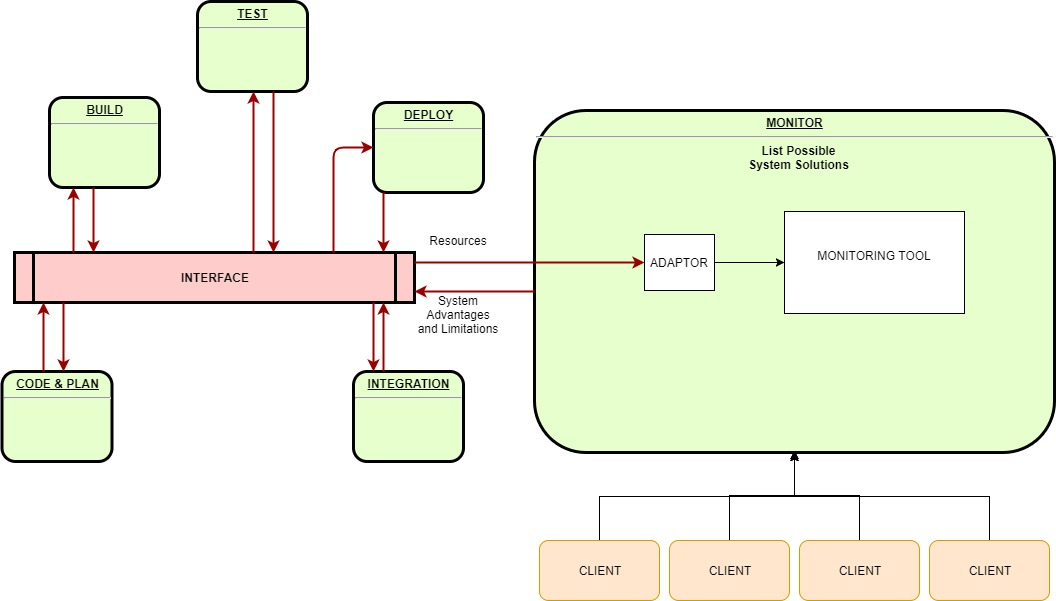
\includegraphics[width=15cm]{uml} %uml
\newline
	\subsection{Product Functions}
GTU CSE343 DevOps Portal Project has a main page which includes six buttons of the parts of DevOps. The last button represents  monitoring. When clicked it redirects to the main page of monitoring that shows the programs that are developed in the portal where you can access the following features by clicking the buttons representing each program. \newline \newline
\newline \newline Monitor: 
 \begin{itemize}
  	\item Application Name : Shows each client that installed the specific application with a representing button.
	 \begin{itemize}
      		\item[$\ast$]{Client Name: Redirects to a new page that has the corresponding information about the client.}	
    \end{itemize}
\end{itemize}

	\subsection{User Classes and Characteristics}
 \begin{itemize}
	\item Developers, who wants to monitor the efficiency of the programs they developed.
	\item Operational users, such as CEO, POs, Scrum Masters, Support Desk, etc. who wants to monitor the clients.
\end{itemize}
	\subsection{Operating Environment}
 \begin{itemize}
 	\item Linux
	\item IBM AIX
	\item FreeBSD
	\item NewBSD
	\item OpenBSD
	\item HP-UX
	\item Mac OS X 
	\item Solaris
	\item Windows: all destop and server versions since 2000 (Zabbix agent only)

\end{itemize}
	\subsection{Design and Implementaion Constraints}
The communication between Interface and Monitoring needs an adapter which is developed in Java. The DevOps Portal Project monitoring module uses Zabbix Monitoring Tool.
	
	\subsection{User Documentation}
This part will be updated according to the progress of the project.

	\subsection{Assumptions and Dependencies}
Since the project uses Zabbix to monitor, it requires every requirement that Zabbix needs such as Apache and PHP which can be accessed from the following link to Zabbix requirements page:
 \MYhref{https://www.zabbix.com/documentation/3.0/manual/installation/requirements}{https://www.zabbix.com/documentation/3.0/manual/installation/requirements}	
Adapters that are used to perform communication between the Interface and the monitor modules are developed in Java therefore Java version 7 or higher has to be installed on the computer that will monitor the clients. 
To access the monitoring module as well as the other modules of the DevOps Portal, a web browser with cookies and JavaScript enabled is required as well.

\section{External Interface Requirements} 

	\subsection{User Interfaces}
This part will be updated according to progress of the project.
	\subsection{Hardware Interfaces}
Memory: \newline    Zabbix requires both physical and disk memory. 128 MB of physical memory and 256 MB of free disk space could be a good starting point. However, the amount of required disk memory obviously depends on the number of hosts and parameters that are being monitored.
\newline \newline
CPU: \newline   Zabbix and especially Zabbix database may require significant CPU resources depending on number of monitored parameters and chosen database engine.
 \newline  More Information:  \MYhref{https://www.zabbix.com/documentation/3.0/manual/installation/requirements}{https://www.zabbix.com/documentation/3.0/manual/installation/requirements}

	\subsection{Software Interfaces}
The project requires Java to be installed on the computer that will monitor. A web browser with cookies and Javascript enabled is required. The system also needs to provide the requirements for Zabbix. Additional information can be found on section 2.7 of this document.
	\subsection{Communications Interfaces}

DevOps Portal Monitoring requires an internet connection and a connection between the clients and the server.

\section{System Features} 

	\subsection{Application Discovery}
This part will be updated according to progress of the project.
	\subsection{Alerts }
This part will be updated according to progress of the project.
	\subsection{Tracking Clients Informations }
This part will be updated according to progress of the project.
	\subsection{Viewing Application Data }
This part will be updated according to progress of the project.
\section{Other Nonfunctional Requirements} 
	\subsection{Performance Requirements }
Memory:\newline 
    Zabbix requires both physical and disk memory. 128 MB of physical memory and 256 MB of free disk space could be a good starting point. However, the amount of required disk memory obviously depends on the number of hosts and parameters that are being monitored.
\newline
CPU:\newline
    Zabbix and especially Zabbix database may require significant CPU resources depending on number of monitored parameters and chosen database engine.

	\subsection{Security Requirements  }
Zabbix does not have any security requirements and thus any type of user can use it without any additional privileges. \newline \newline
\section{Glossary} 
\begin{itemize}
	\item	Adapter: In computing, adapter is a hardware or software device that converts transmitted data from one presentation form to another.
	\item 	Client: A client is a piece of computer hardware or software that accesses a service made available by a server.
 	\item Cookies: Small files which are stored on a user's computer. They are  designed to hold a modest amount of data specific to a particular client and website, and can be accessed either by the web server or the client computer.
	\item DevOps: It is a project development philosophy which aims at increasing software         
            productivity by combining development and Operational part of project  together.
	\item GTU: An acronym for Gebze Technical University.
	\item Server: In computing, a server is a computer program or a device that provides functionality for other programs or devices, called “clients”.

	\item	Web Browser: A web browser is a software application for retrieving, presenting and traversing information resources on the Word Wide Web.
	\item	Zabbix: An open source application monitoring tool.

\end{itemize}


	
	


\end{document}
